\documentclass[tikz,border=3pt]{standalone}
\usetikzlibrary{arrows.meta}
\begin{document}
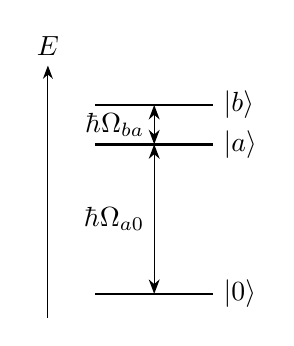
\begin{tikzpicture}[scale=1.0,>=Stealth,line width=0.9pt]
  % 縦軸（エネルギー）
  \draw[line width=0.4pt,->] (0,0) -- (0,3.2) node[above] {$E$};

  % エネルギー準位 |0>, |a>, |b>
  \draw (0.6,0.3) -- (2.1,0.3) node[right] {$|0\rangle$};
  \draw (0.6,2.2) -- (2.1,2.2) node[right] {$|a\rangle$};
  \draw (0.6,2.7) -- (2.1,2.7) node[right] {$|b\rangle$};

  % エネルギー差の矢印
  \draw[line width=0.5pt,<->] (1.35,0.3) -- (1.35,2.2) node[midway,left] {$\hbar\Omega_{a0}$};
  \draw[line width=0.5pt,<->] (1.35,2.2) -- (1.35,2.7) node[midway,left] {$\hbar\Omega_{ba}$};
\end{tikzpicture}
\end{document}
